% Created 2016-02-19 Fri 12:33
\documentclass[11pt]{article}
\usepackage[utf8]{inputenc}
\usepackage[T1]{fontenc}
\usepackage{fixltx2e}
\usepackage{graphicx}
\usepackage{grffile}
\usepackage{longtable}
\usepackage{wrapfig}
\usepackage{rotating}
\usepackage[normalem]{ulem}
\usepackage{amsmath}
\usepackage{textcomp}
\usepackage{amssymb}
\usepackage{capt-of}
\usepackage{hyperref}
\author{Gun Woo Park}
\date{\today}
\title{Data Structure and Travel Algorithm}
\hypersetup{
 pdfauthor={Gun Woo Park},
 pdftitle={Data Structure and Travel Algorithm},
 pdfkeywords={},
 pdfsubject={},
 pdfcreator={Emacs 24.5.1 (Org mode 8.3.1)}, 
 pdflang={English}}
\begin{document}

\maketitle
\tableofcontents


\section{Preface}
\label{sec:orgheadline1}
This documentation is related with the basic data structure and travel algorithm for the given graph structure in order to identify percolated structure. 

\section{Multi-dimensional Array}
\label{sec:orgheadline2}
For compatibility and convenience, the multi-dimensional arrays are expressed by one-dimensional array by index mapping function. To be specific, the given N by M 2-dimensional array may have the form of table \ref{tab:orgtable1}, which is possibly mapped to table \ref{tab:orgtable2}. The advantage for this expression can be thought as two parts: coding interface can be united and we can use several compression techniques such as lower occupation for symmetric matrix. There are various numerical packages have been used this way: BLAS, LAPACK, GSL, and so on.


\begin{table}[htb]
\caption{\label{tab:orgtable1}
Example for typical 2-dimensional array}
\centering
\begin{tabular}{cccccc}
index & 0 & 1 & 2 & \(\cdots\) & M\\
\hline
0 & val(0,0) & val(0,1) & val(0,2) &  & val(0, M)\\
1 & val(1,0) & val(1,1) & val(1,2) &  & val(1, M)\\
 &  & \(\vdots\) &  & \(\ddots\) & \\
N & val(N,0) & val(N,1) & val(N,2) &  & val(N,M)\\
\end{tabular}
\end{table}

\begin{table}[htb]
\caption{\label{tab:orgtable2}
Example for mapping to 1-dimensional array from 2-dimensional array.}
\centering
\begin{tabular}{cccccccc}
index & 0 & 1 & \(\cdots\) & M & M+1 & \(\cdots\) & NM\\
\hline
coord. & (0,0) & (0,1) & \(\cdots\) & (0,M) & (1,0) & \(\cdots\) & (N,M)\\
\hline
val. & val(0,0) & val(0,1) & \(\cdots\) & val(0,M) & val(1,M) & \(\cdots\) & val(N,M)\\
\end{tabular}
\end{table}



\section{Adjacency Matrix and List}
\label{sec:orgheadline3}
Consider the given association information, we can easily express the information using adjacency matrix:
\begin{equation}
\mathbf{C}_m = \left[\mathscr{C}_{ij}\right],
\end{equation}
where \(\mathscr{C}_{ij}\) is number of associations for the pair of i- and j-th particles.
The expression is quite simple and it contains all the existing information. However, the adjacency matrix is expensive both of time and space complex because adjacency matrix explicitly denote zeros inside the array, which needed more time for zero identification during processing. Hence, the adjacency list have been used :
\begin{equation}
\mathbf{C}_l = \left[\mathscr{I}_{i}(j)\right],
\end{equation}
where i denote the index for subject particle, j denote index for columns, and \(\mathscr{I}_{i}(j)\) is the index that is j-th connection to the i-th particle. 
For instance, consider the given network has the form of figure \ref{orgkeyword1}, then the adjacency matrix becomes table \ref{tab:orgtable3} and the adjacency list is expressed in table \ref{tab:orgtable4}. Note that the weight for the bridge should be stored in separated array for adjacency list.

\begin{figure}[htb]
\centering
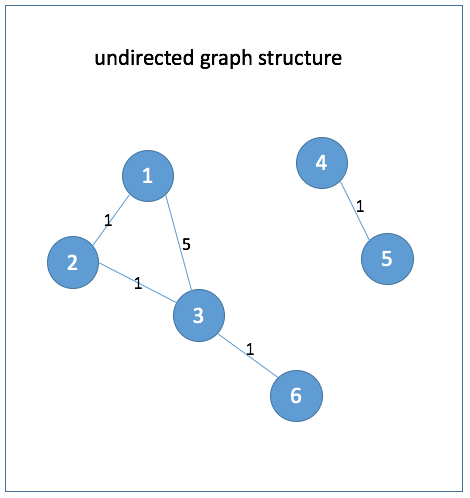
\includegraphics[width=.9\linewidth]{data_structure/ex_graph_association.png}
\caption{Example for association maps. It can be regarded as undirected graph since there is no directional information for the association (edge as CS notation) between particles (vortex as CS notation).}
\end{figure}


\begin{table}[htb]
\caption{\label{tab:orgtable3}
Example of adjacency matrix for figure \ref{orgkeyword1}.}
\centering
\begin{tabular}{rrrrrrr}
 & 1 & 2 & 3 & 4 & 5 & 6\\
\hline
1 & \(N_1\) & 1 & 5 & 0 & 0 & 0\\
\hline
2 & 1 & \(N_2\) & 1 & 0 & 0 & 0\\
\hline
3 & 5 & 1 & \(N_3\) & 0 & 0 & 1\\
\hline
4 & 0 & 0 & 0 & \(N_4\) & 1 & 0\\
\hline
5 & 0 & 0 & 0 & 1 & \(N_5\) & 0\\
\hline
6 & 0 & 0 & 1 & 0 & 0 & \(N_6\)\\
\end{tabular}
\end{table}

\begin{table}[htb]
\caption{\label{tab:orgtable4}
Example of adjacency list for figure \ref{orgkeyword1}.}
\centering
\begin{tabular}{rrrr}
bead & 0 & 1 & 2\\
\hline
1 & 2 & 3 & 0\\
2 & 1 & 3 & 0\\
3 & 1 & 2 & 6\\
4 & 5 & 0 & 0\\
5 & 4 & 0 & 0\\
6 & 3 & 0 & 0\\
\end{tabular}
\end{table}


\section{Identification for Percolation}
\label{sec:orgheadline13}
The percolation for one spatial dimension can be solved by travel algorithm for undirected graph structure in the word of computer science. The idea is to travel through all the bridge that connected the subjected particle, then identify the travel goes beyond box or not. 






\subsection{Travel Beyond Box Boundary}
\label{sec:orgheadline6}
\subsubsection{Minimum Image Convention}
\label{sec:orgheadline4}
Before going further, it is better to mention that the minimum distance between particles in periodic boundary condition (PBC) is using component-wise minimization:
\begin{equation}
\label{eq:orglatexenvironment1}
r^{(m)}_k(\mathbf{r}_i, \mathbf{r}_j) = \min\left\{x_k(\mathbf{r}_j) - \left(L_D\mathscr{S} + x_k(\mathbf{r}_i)\right)\right\},
\end{equation}
where \(k\) denote the k-th spatial dimension and \(L_D\) is box dimension and the shift set is given by \(\mathscr{S} = \{-1, 0, +1\}\),
which implies the relative vector of minimum distance from \(\mathbf{r}_j\) to \(\mathbf{r}_i\) is
\begin{equation}
Crd_{\varepsilon}\left(\mathbf{r}^{(m)}(\mathbf{r}_i, \mathbf{r}_j)\right) = [r_1(\mathbf{r}_i, \mathbf{r}_j), \cdots, r_{N_D}(\mathbf{r}_i, \mathbf{r}_j)]^T,
\end{equation}
where \(\varepsilon\) is given basis set. Minimum distance is simply given by Euclidean norm of this relative vector of minimum distance.

\begin{figure}[htb]
\centering
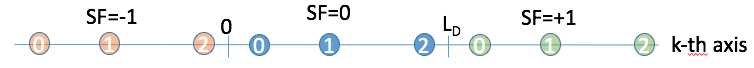
\includegraphics[width=.9\linewidth]{data_structure/comp_minimum_distance.png}
\caption{Component-wise minimum distance relative vector}
\end{figure}

Let assume that we have 3 particles and the subject particle is zero, which depicted figure \ref{orgkeyword2}. If we started with 0th particle and try to find its the minimum distance with 2nd particle. For this processing, we have to count its the images of 2nd particle which can be in left or right side. The meaning of real left and right is not important because the axis independence. This is exactly the same meaning with equation \ref{eq:orglatexenvironment1} since
\begin{equation}
d^{(m)}_{ij} = \left|\mathbf{r}^{(m)}(\mathbf{r}_i, \mathbf{r}_j)\right|_2 = \sqrt{\sum_{k=1}^{N_d} (r^{(m)}_k(\mathbf{r}_i, \mathbf{r}_j))^2}
\end{equation}
becomes minimum when each \(r^{(m)}_k\) is minimum. Notice that this happens because of orthonormal basis. \emph{For general basis set, it is of importance that we have to measure component based on reciprocal base vector, which will be involved when the system is experienced shear.} 

\subsubsection{Identifier for Boundary Travels and Percolation}
\label{sec:orgheadline5}
For each travels, we can count shift factor for individual axis. If all the shift factors are zeros, it means the travel will happen inside of box. If k-th dimension has left (-1) or right (+1) shift factor, then the given travel goes beyond left or right boundary of k-th axis, respectively. In one cluster, the percolation through k-th axis happens when it travel both of left and right boundary.

\subsection{Travel Algorithm}
\label{sec:orgheadline11}
\subsubsection{Travel for Vertex: Measuring Cluster Size Distribution}
\label{sec:orgheadline7}
Let say cluster as the group of particles that is connected. The size of cluster is defined by number of particles on the subjected cluster, then we can measure cluster size distribution of given system. 

The given associated network has the same structure with the undirected graph that is composed of vertexes (particles in this case) and edges (association in this case). Undirected means that bridge chain is symmetric under the index of pair of particles, \(\mathbf{r}_{ij} = \mathbf{r}_{ji}\). Extracting information of association topology is done through traveling the network and the data is given by adjacency list. In general, depth-first search (DFS) and breadth-first search (BFS) are good for this aspect with different spanning tree. The details of the data structure and algorithm are described on Appendix. 



\subsubsection{Travels for Edges: Identify Travels Beyond PBC Box}
\label{sec:orgheadline8}
Travel for vertex means we visit all the particles that connected with the given root particle, but it does not guarantee that visiting all the edges (bridges). The percolation identification depends on the bridges, not about particles itself, which means we need to modify travel algorithm. There are various way to travel edges rather than vertex, but we need only information of edge not about real travels. Hence, the algorithm is slightly modified to record the identifier for shift factor for all the possible travel path - but do not act the travel when the target particle is already in-visited status. 

\subsubsection{Travels inside PBC Box}
\label{sec:orgheadline9}
As already mentioned in above, the travel is only allowed inside box and whenever travel is experienced beyond box, travel is canceled and it will be recorded for percolation identification. To be specific, consider the networks in figure \ref{fig:orgparagraph1} shows that different percolation scheme. However, the percolation through x axis in the (b) of figure \ref{fig:orgparagraph1} cannot be captured by given scheme since the percolation line through the boundary of subjected box. For relatively large 3-dimensional box, the situation is not so common, which is the reason to use introduced identification procedure. 

\begin{figure}[htb]
\centering
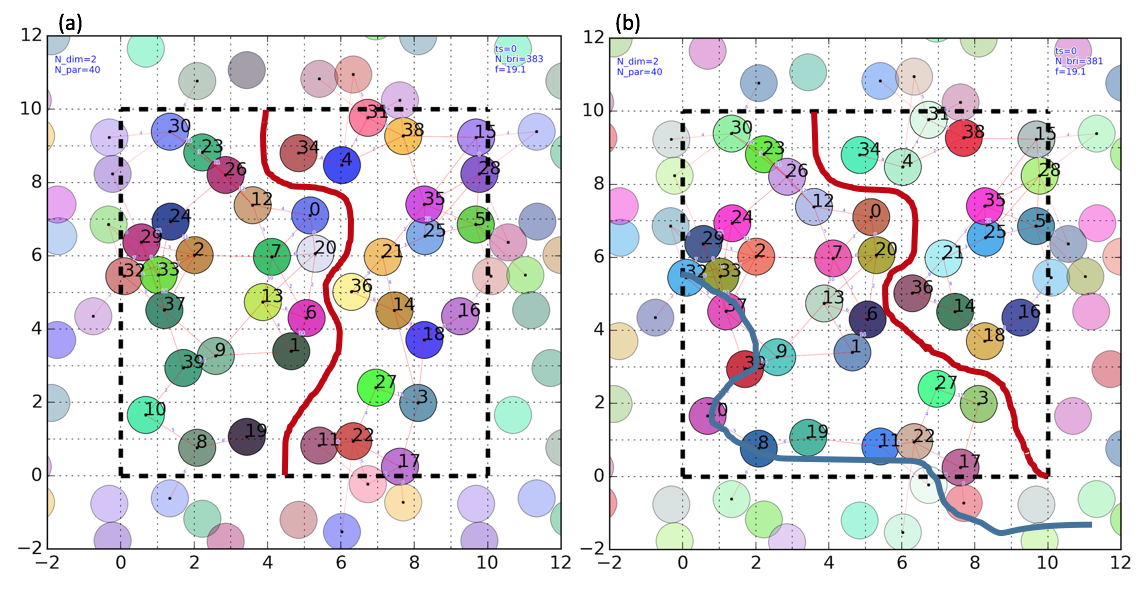
\includegraphics[width=.9\linewidth]{data_structure/ex_percolation_identification.png}
\caption{\label{fig:orgparagraph1}
Two dinsintuishable 2-dimensional cluster system. Left figure (a) represent percolation happens along y axis while no percolation along x axis. Right figure (b) represent the percolation happens both of x and y axis, but x percolation line beyond the subjected box. The thick red line represent isolation while the thick blue line represent percolation line along x axis.}
\end{figure}

It also works well for 3-dimensional case. The given association information depicted in \ref{fig:orgparagraph2}. By eyes, it is not easy to judge there exist percolation cluster or not. From this algorithm, it reveals that the root index 0 is composed of 191 pairs of association that percolated along all the axis: x, y, and z. If we measure cluster size distribution and identify the given cluster is percolated with specified axis or not, the figure \ref{fig:orgparagraph3} is good point to observe. There are 60 distinguishable clusters and 2122 total number of particles in 60 clusters. Since the number of distinguishable association is 6022, 3900 particles are isolated or attached to wall. For detail distribution, the travel should be allowed for directed image (which will be implemented later) then the distribution will be more accurate.

\begin{figure}[htb]
\centering
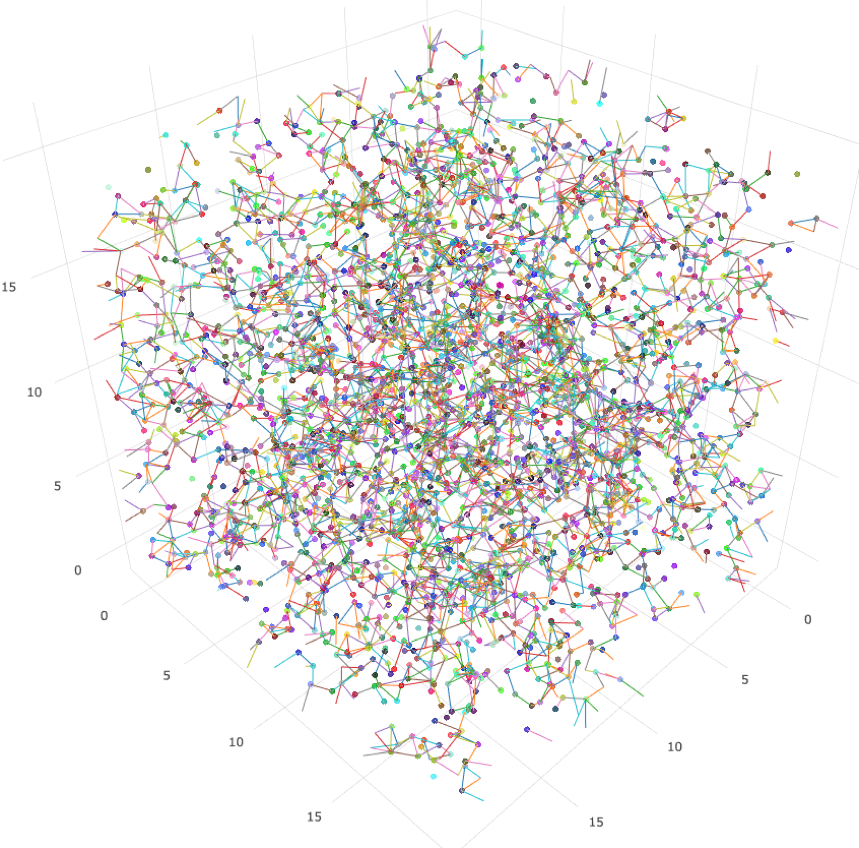
\includegraphics[width=.9\linewidth]{data_structure/ex_3d_NP3200_SF20_percolation.png}
\caption{\label{fig:orgparagraph2}
Equilibrium topology with the given condition: 3200Np, \(20^3\) dimensionless volume, 25 chains per each particle. Re-scaling factor is used 2.0.}
\end{figure}

\begin{figure}[htb]
\centering
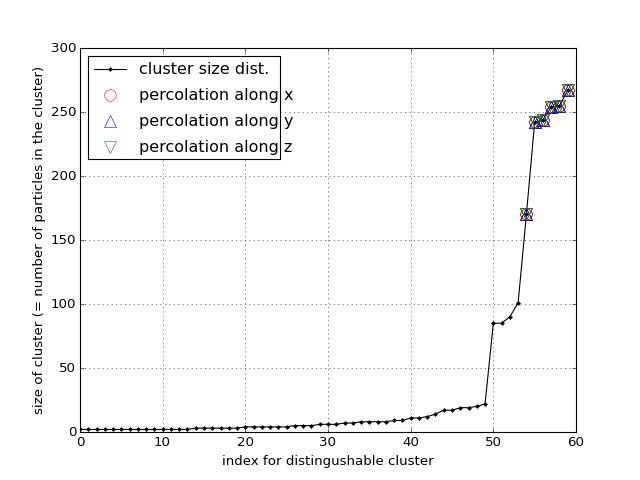
\includegraphics[width=.9\linewidth]{data_structure/percolation_test_3D.png}
\caption{\label{fig:orgparagraph3}
Cluster size distribution and identification for percolation with each independent axis.}
\end{figure}



\subsubsection{{\bfseries\sffamily TODO} Allowing Travel Beyond Boundary of Box}
\label{sec:orgheadline10}
Notice that the following article is description for the idea. The alogirthm is not fully implemented into sourcecode, which will achieve later progress.

It might be more general way to allow travel beyond boundary of box. At this moment, there are several difficulties to allow such a travels. The most importance question is \emph{how to identify percolation}.

Allowing one more image of the subjected box is a key to identify percolation. During travels, we have to record all the parity of the travel identifier since it is a key of image. Sum of all travel identifier for a given axis, say image identifier, should not lower than -1 and higher than +1, which means only direct image of subjected box will be accounted. It is of importance to distinguish between particles in different box even if they have the same index number, which can be achieved using image identifier:
\begin{equation}
I^{k} = \sum_{i=1}^{N_{tb}} s^{k}_i,
\end{equation}
where \(N_{tb}\) is number of travel beyond boundary, k denote k-th spatial dimension and \(s^k_i \in \mathscr{S}\). It is quite simple that the image identifier, \(I^{k}\) can be any value of \(\mathscr{S}=\{-1, 0, +1\}\), which direct the current travel happens in the left, center, or right side of the box, respectively. Therefore, \emph{recorded shift factor is not the instance shift factor but sum of all instance shift factors.} Note that the travel to image particle is allowed even if its original particle in current PBC box is visited status. Once the travel is finished, all the particles in its direct image have been visited status and we have to make sure the all the edges are accounted for identification of travel. 

The identifier for this case is the same with travel identifier inside box: one cluster for k-th axis shows both of left and right imaginary shift factor, this is percolated. We do not need to travel further from direct image of current box. For simplification, the index vector is introduce:
\begin{equation}
\mathbf{I} = [i_1, i_2, i_3]^T,
\end{equation}
where \(i_1, i_2, i_3\) are the index for each axis. If the subjected particle is in current PBC box, the components are \(i_1 = i_2 = i_3 = i\) where i is the original index for the particle. If it is in directed image of PBC box, we can use shifted index:
\begin{equation}
i_k = i + S_k N_p,
\end{equation}
where \(S_k\) is the shift factor for the given axis and \(N_p\) is number of particles. For instance, if the system has 10 particles inside PBC box, then the \(i_k\) value becomes -10 to 20: -10 to -1 for the left image of k-th axis, 0 to 10 for the current box, and 11 for 20 for the right image of k-th axis. The mapping function from image of box to current box is easily given by \(i_k\) modulo \(N_p\): \(i_k\% N_p\). This benefit to record and tracking the stack memory of the iterative DFS algorithm.










\subsection{Python Code for Measuring Cluster Size and Percolation Identification}
\label{sec:orgheadline12}
There are various way to develop DFS algorithm for tree structure in general way. It is quite simple to use recursive form since DFS is using call stack. With given size of cluster, however, the recursive call is limited by system for safety reason, and have potential overhead because of calling functions typically taking time. On this regards, the code is developed by iterative manner with some set of if-phrase in order to identify edge travels. The code is described on code \ref{orgsrcblock1} written by python. The root index will be given by the argument index (default is zero). When we need to travel all the sub-graph of given graph (existing several clusters), we can iterate root index from zero to number of particles, then we can extract distinguishable clusters, which is the way to measure cluster size distribution.



\section{Appendix}
\label{sec:orgheadline16}
\subsection{Graph}
\label{sec:orgheadline14}
Mathematically, a graph is an ordered pair \(G = (V, E)\) where a set \(V\) of vertices and a set \(E\) of edges. 

For instance, we have vertices and edges for figure \ref{orgkeyword3} as 
\begin{align}
V &= \{0, 1, 2, 3, 4, 5\}\\
E &= \{(0, 1), (0, 3), (1, 2), (2, 4), (2, 5), (3, 4), (4, 5)\},
\end{align}
which in consequence \(V\) is set of all the index for particles and \(E\) is set of all pairs of index for bridges. It is of importance that the identification of percolation is not necessary to count weight on the bridge, i.e., number of connections for the same bridge, so we do not need count all the weight array on this graph analysis. In addition, the given graph is undirected since all the element for \(E\) is symmetric under the pair index: \((i, j) = (j, i)\). 

\begin{figure}[htb]
\centering
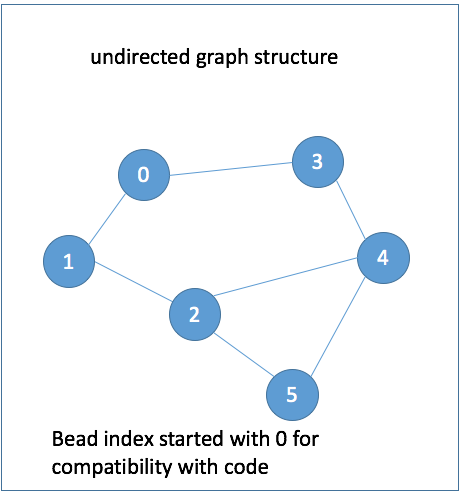
\includegraphics[width=.9\linewidth]{data_structure/ex_graph_DFS.png}
\caption{Example for association maps. This example will be used DFS testing and the starting index  changed to 0 from 1 for compatibility with the code infrastructure. Therefore, index zero indicate the zero-th particle and -1 indicate there is no association.}
\end{figure}

\subsection{Tree and Spanning Tree}
\label{sec:orgheadline15}
Tree is linearized graph, which means graph without any circle of bridges. For given network structure is not tree because of association can happens to make loop. To understand tree structure, however, is of importance since the algorithms to travel graph is based on the tree. Basically, the graph cannot be merged to tree structure, but if we ignore loop bridges, we can span tree structure from given graph which is called \emph{spanning tree}. In consequence of linearization, the spanning tree is not unique that depends on the algorithms to travel. 

To be specific, for graph depicted in figure \ref{orgkeyword3}, if we apply DFS algorithm, the spanning tree has the form of figure \ref{orgkeyword4}. Here, the 0-th particle is selected as root, and the rank of child is represented by depth from root. If we use BFS algorithm, the spanning tree has different form like figure \ref{orgkeyword5}. The travel sequence for DFS becomes \(0\to 1\to 2\to 4\to 3\to 5\) while BFS becomes \(0\to 1\to 3\to 2\to 4\to 5\). In principle, the spanning tree is not necessary to generate but it is good way to understand the properties of given graph. Since DFS is used as default, this article only contains details about DFS. The adjacency list for the given graph is described in table \ref{tab:orgtable5}.

\begin{table}[htb]
\caption{\label{tab:orgtable5}
Adjacency list for the given graph, figure \ref{orgkeyword3}}
\centering
\begin{tabular}{rrrr}
 & 1 & 2 & 3\\
\hline
0 & 1 & 3 & -1\\
1 & 0 & 2 & -1\\
2 & 1 & 4 & 5\\
3 & 0 & 4 & -1\\
4 & 2 & 3 & 5\\
5 & 2 & 4 & -1\\
\hline
\end{tabular}
\end{table}



\begin{figure}[htb]
\centering
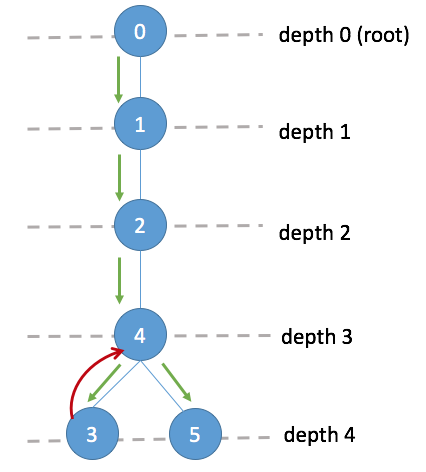
\includegraphics[width=.9\linewidth]{data_structure/spanning_tree_DFS.png}
\caption{DFS spanning tree for graph depicted in figure \ref{orgkeyword3}.}
\end{figure}

\begin{figure}[htb]
\centering
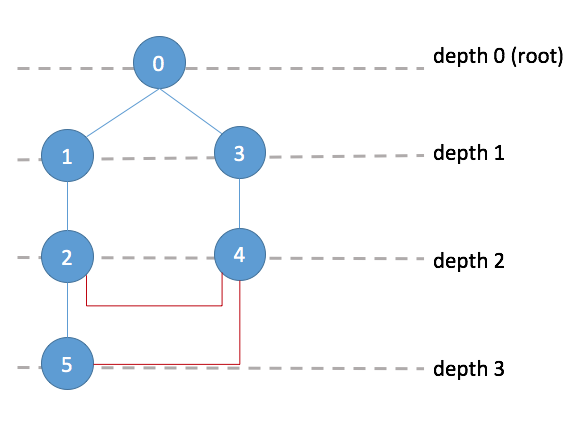
\includegraphics[width=.9\linewidth]{data_structure/spanning_tree_BFS.png}
\caption{BFS spanning tree for graph depicted in figure \ref{orgkeyword3}.}
\end{figure}



\section{Codes}
\label{sec:orgheadline19}

\subsection{Component-wise Minimum Distance}
\label{sec:orgheadline17}
\begin{verbatim}
1  double get_minimum_image_k_from_x(double x, double k, double dimension)
2  {
3      double kd[3] = {k-dimension - x, k - x, k + dimension - x};
4      double re = [get_index_minimum_abs(kd, 3)] + x;
5      return re;
6  }
\end{verbatim}

\subsection{DFS for identification of percolation}
\label{sec:orgheadline18}
\begin{verbatim}
 1  def check_travel_beyond_box(pos, index, target, Ld):
 2      Nd = shape(pos)[1]
 3      for k in range(Nd):
 4          if (ident_minimum_distance_k_from_x(pos[index, k], pos[target, k], Ld) != 0):
 5              return 1
 6      return 0
 7  
 8  def ident_minimum_distance_k_from_x(x, k, box_dimension):
 9      kd = asarray([k-box_dimension - x, k-x, k+box_dimension-x])
10      return argmin(abs(kd)) - 1 # will return [-1, 0, +1]
11  
12  def ident_over(hash, index, order_count):
13      N_cols = shape(hash)[1]
14      if order_count >= N_cols:
15          return 1
16      if int(hash[index, order_count]) is -1:
17          return 1
18      return 0
19  
20  def cluster_edge_DFS_travel_restricted_box_iter(hash, pos, Ld, record_component, index=0, order_count=1, cnt=0, IDPC=[], IDPI=[], stack=[], stack_order=[]):
21      cnt = 0; const_new_order_count = 1 # initialisation variables
22      N_cols = shape(hash)[1] # limitation for the hash tables
23      stack.append(int(index)); stack_order.append(order_count) # initial stacking
24      while(size(stack) > 0): # will false when size(stack) is 0 if it is not initial step
25          cnt += 1 # temporal counting 
26          ident_over_cols = ident_over(hash, index, order_count)
27          if ident_over_cols: # in the case that the hash[index, order_count] reaching end (-1 or order_count is over)
28              stack = stack[:-1]; stack_order = stack_order[:-1]
29              if (size(stack) > 0):
30                  index = stack[-1]; order_count = stack_order[-1] + 1
31          else: # in the case that the hash[index, order_count] is properly defined
32              target = hash[index, order_count]
33              travel_beyond_box = check_travel_beyond_box(pos, index, target, Ld)
34              if (target in record_component) or travel_beyond_box: # when target is in stack stack or travel beyond box boundary
35                  if travel_beyond_box: 
36                      for id in range(shape(pos[index, :])[0]):
37                          ident_IDP = ident_minimum_distance_k_from_x(pos[index, id], pos[target, id], Ld)
38                          if (int(ident_IDP) is not 0) and ([index, target] not in IDPI):
39                              IDPC.append([id, ident_IDP])
40                              IDPI.append([index, target])
41                  # when particle is duplicated or travel_beyond_box
42                  index = index; order_count = order_count + 1;
43  
44                  # this means it inherit the exist index for bead but increase order_count
45                  # note that the target for next step is given by hash[index, order_count]
46              else: # when the target will stack
47                  record_component.append(int(target))
48                  stack.append(int(target)); stack_order.append(order_count) # record element and its order for stack
49                  index = target; order_count = const_new_order_count; # depth first search
50      return size(stack)
\end{verbatim}
\end{document}